%%%%%%%%%%%%%%%%%%%%%%%%%%%%%%%%%%%%%%%%%
% Proceedings of the National Academy of Sciences (PNAS)
% LaTeX Template
% Version 1.0 (19/5/13)
%
% This template has been downloaded from:
% http://www.LaTeXTemplates.com
%
% Original author:
% The PNAStwo class was created and is owned by PNAS:
% http://www.pnas.org/site/authors/LaTex.xhtml
% This template has been modified from the blank PNAS template to include
% examples of how to insert content and drastically change commenting. The
% structural integrity is maintained as in the original blank template.
%
% Original header:
%% PNAStmpl.tex
%% Template file to use for PNAS articles prepared in LaTeX
%% Version: Apr 14, 2008
%
%%%%%%%%%%%%%%%%%%%%%%%%%%%%%%%%%%%%%%%%%

%----------------------------------------------------------------------------------------
%	PACKAGES AND OTHER DOCUMENT CONFIGURATIONS
%----------------------------------------------------------------------------------------

%------------------------------------------------
% BASIC CLASS FILE
%------------------------------------------------

%% PNAStwo for two column articles is called by default.
%% Uncomment PNASone for single column articles. One column class
%% and style files are available upon request from pnas@nas.edu.

%\documentclass{pnasone}
\documentclass{pnastwo}

%------------------------------------------------
% POSITION OF TEXT
%------------------------------------------------

%% Changing position of text on physical page:
%% Since not all printers position
%% the printed page in the same place on the physical page,
%% you can change the position yourself here, if you need to:

% \advance\voffset -.5in % Minus dimension will raise the printed page on the 
                         %  physical page; positive dimension will lower it.

%% You may set the dimension to the size that you need.

%------------------------------------------------
% GRAPHICS STYLE FILE
%------------------------------------------------

%% Requires graphics style file (graphicx.sty), used for inserting
%% .eps/image files into LaTeX articles.
%% Note that inclusion of .eps files is for your reference only;
%% when submitting to PNAS please submit figures separately.

%% Type into the square brackets the name of the driver program 
%% that you are using. If you don't know, try dvips, which is the
%% most common PC driver, or textures for the Mac. These are the options:

% [dvips], [xdvi], [dvipdf], [dvipdfm], [dvipdfmx], [pdftex], [dvipsone],
% [dviwindo], [emtex], [dviwin], [pctexps], [pctexwin], [pctexhp], [pctex32],
% [truetex], [tcidvi], [vtex], [oztex], [textures], [xetex]

\usepackage{graphicx}

%------------------------------------------------
% OPTIONAL POSTSCRIPT FONT FILES
%------------------------------------------------

%% PostScript font files: You may need to edit the PNASoneF.sty
%% or PNAStwoF.sty file to make the font names match those on your system. 
%% Alternatively, you can leave the font style file commands commented out
%% and typeset your article using the default Computer Modern 
%% fonts (recommended). If accepted, your article will be typeset
%% at PNAS using PostScript fonts.

% Choose PNASoneF for one column; PNAStwoF for two column:
%\usepackage{PNASoneF}
%\usepackage{PNAStwoF}

%------------------------------------------------
% ADDITIONAL OPTIONAL STYLE FILES
%------------------------------------------------

%% The AMS math files are commonly used to gain access to useful features
%% like extended math fonts and math commands.

\usepackage{amssymb,amsfonts,amsmath}
\usepackage[]{algorithm2e}

%------------------------------------------------
% OPTIONAL MACRO FILES
%------------------------------------------------

%% Insert self-defined macros here.
%% \newcommand definitions are recommended; \def definitions are supported

%\newcommand{\mfrac}[2]{\frac{\displaystyle #1}{\displaystyle #2}}
%\def\s{\sigma}

%------------------------------------------------
% DO NOT EDIT THIS SECTION
%------------------------------------------------

%% For PNAS Only:
\contributor{Submitted for Applied Mathematics 205, Harvard University}
\url{Zhang and Zochowski}
\copyrightyear{2014}
\issuedate{}
\volume{Spring}
\issuenumber{}

%----------------------------------------------------------------------------------------

\begin{document}

%----------------------------------------------------------------------------------------
%	TITLE AND AUTHORS
%----------------------------------------------------------------------------------------

\title{PDE-based interpolation for image compression} % For titles, only capitalize the first letter

%------------------------------------------------

%% Enter authors via the \author command.  
%% Use \affil to define affiliations.
%% (Leave no spaces between author name and \affil command)

%% Note that the \thanks{} command has been disabled in favor of
%% a generic, reserved space for PNAS publication footnotes.

%% \author{<author name>
%% \affil{<number>}{<Institution>}} One number for each institution.
%% The same number should be used for authors that
%% are affiliated with the same institution, after the first time
%% only the number is needed, ie, \affil{number}{text}, \affil{number}{}
%% Then, before last author ...
%% \and
%% \author{<author name>
%% \affil{<number>}{}}

%% For example, assuming Garcia and Sonnery are both affiliated with
%% Universidad de Murcia:
%% \author{Roberta Graff\affil{1}{University of Cambridge, Cambridge,
%% United Kingdom},
%% Javier de Ruiz Garcia\affil{2}{Universidad de Murcia, Bioquimica y Biologia
%% Molecular, Murcia, Spain}, \and Franklin Sonnery\affil{2}{}}

\author{Andrew Wang\affil{1}{awang@college.harvard.edu}
\and
Kevin Zhang\affil{2}{kzhang@college.harvard.edu}}

\contributor{Submitted as a final project for Applied Mathematics 205}

%----------------------------------------------------------------------------------------

\maketitle % The \maketitle command is necessary to build the title page

\begin{article}

%----------------------------------------------------------------------------------------
%	ABSTRACT, KEYWORDS AND ABBREVIATIONS
%----------------------------------------------------------------------------------------

\begin{abstract}
We review the mathematical basis behind PDE-based image editing, focusing on methods of image interpolation for inpainting, including smoothing, linear diffusion, and nonlinear diffusion. Additionally, we implement a PDE-based image compression and decompression scheme. We investigate random sampling and a recursive tree-based sampling method for selecting pixels to decompress.
\end{abstract}

%------------------------------------------------

\keywords{Image Editing | PDE | Compression | Interpolation | Inpainting | BTTC} % When adding keywords, separate each term with a straight line: |

%------------------------------------------------

%% Optional for entering abbreviations, separate the abbreviation from
%% its definition with a comma, separate each pair with a semicolon:
%% for example:
%% \abbreviations{SAM, self-assembled monolayer; OTS,
%% octadecyltrichlorosilane}

% \abbreviations{}
\abbreviations{BTTC, B-tree triangular coding; PDE, partial differential equation; RGB, red-blue-green; 
EED, edge-enhancing diffusion; MSE, mean-squared error}

%----------------------------------------------------------------------------------------
%	PUBLICATION CONTENT
%----------------------------------------------------------------------------------------

%% The first letter of the article should be drop cap: \dropcap{} e.g.,
%\dropcap{I}n this article we study the evolution of ''almost-sharp'' fronts

\section{Introduction}

\dropcap{L}ossy compression is a data encoding method that aims to reduce the redundancy of a data file so that it can be stored and transmitted efficiently.  Lossy compression techniques are especially important for multimedia applications such as image compression due to the large file sizes involved.  For example, a 1 megapixel photo with 24 bits per pixel---8 bits per color---requires at least 3 megabytes to store in raw form.  Lossy compression involves discarding some of the total information in the data to substantially reduce its size (in contrast to lossless compression, which preserves all information).  Many popular image formats, including the JPEG family, use lossy compression and can typically reduce file size by upwards of 80\% before degradation is noticeable.

%The most popular lossy compression approach for images uses wavelet or discrete cosine transforms.  
The most popular established image compression standards, including JPEG and JPEG 2000, typically use wavelet transforms and frequency quantization.  However, these classical image compression usually have ``blind'' steps that unnecessarily introduce loss of information.  JPEG, for instance, chops the image into $8 \times 8$ pixel blocks that are transformed into a frequency domain via a discrete cosine transform, which can lead to the blocky compression artifacts typical of a highly compressed JPEG image (see Fig. \ref{jpegfig}).  On the other hand, image compression methods based on partial differential equations (PDEs) constitute a relatively new class of lossy compression techniques that have the ability to use image features like corners.  The PDE approach involves representing an image with a small subset of data points on the spatial domain which can then be used to reconstruct the image via PDE-based interpolation techniques.  Due to the variety of linear and nonlinear PDEs that can be easily substituted into this framework, the PDE approach offers flexibility for both efficiency and accuracy. \cite{zimmer}.

\begin{figure*}[!htb]
\begin{center}
\includegraphics[width=2in]{JPEG_example_100.jpg}\qquad
\includegraphics[width=2in]{JPEG_example_001.jpg}
\caption{JPEG compression artifacts.  The original image on left is compressed using JPEG at a rate of 1:100, leading to noticeable artifacts in the compressed image on the right. This demonstrates the need for less ``blind'' lossy compression formats. \cite{jpeg}}
\label{jpegfig}
\end{center}
\end{figure*}

We will implement an image compression format using PDEs in \textsc{Matlab}.  The overall approach utilizes PDE-based interpolation on a subset of original image data to reconstruct the image as best as possible (a process called \emph{inpainting}). Our implementation consists of three components: (1) a compression algorithm to select the points, (2) a storage format to store the points and associated data, and (3) a decompression algorithm to reconstruct the original image.  For our purposes, steps (1) and (3) are of particular interest due to their relevance to scientific computing.  For compression (1), we will use \emph{B-tree triangular coding (BTTC)}, a tree-based method that decomposes an image into triangles to identify significant \emph{corners}.  Corners are of particular interest because they occur where the edges of the image change direction, and thus allow for the identification of regions of change within the image without needing the redundancy of storing edges.  For storage (2), we will save the flattened indices and color values of the selected points in a matrix. For decompression (3), we will examine a variety of linear and non-linear PDEs to interpolate the compressed data.


\section{Images as functions}

In order to describe the approach mathematically, we represent images as functions.  An image with $c$ channels is a function $u: \Omega \rightarrow \mathbb{R}^c$, where $\Omega \subset \mathbb{R}^n$ is an $n$-dimensional image domain.  For our purposes, we will use color images with three channels for RGB such that $c = 3$ and $n = 2$.  In this framework, images take in a point $(x,y) \in \Omega$ and return an RGB triple.  A major benefit of the functional representation of images is that it allows for the use of image derivatives that will form the basis of the PDEs.  For example, an image $u : \Omega \rightarrow R$ has a partial derivative with respect to $x$ of $\partial_x u := u_x$ and a gradient $\nabla u$.

Since the image functions are continuous but the image data is discrete, we must discretize the functional framework to apply it practically.  For an image $u$, we have a discrete pixel grid data matrix with width $N_1$ and height $N_2$.  If the image has width $a_1$ and height $a_2$ (i.e. support of $\Omega$ on $(0, a_1) \times (0,a_2)$), then the grid size is $h_1 = a_1 / N_1$ in the $x$-direction and $h_2 = a_2 / N_2$ in the $y$-direction.  To discretize the image, we transfer the continuous image domain $\Omega \in \mathbb{R}^2$ to the rectangular discrete domain $\Omega_{\text{dis}} = \{0,\dots,N_1-1\} \times \{0,\dots,N_2-1\}$ (sampling) and discretize the co-domain of image values $\mathbb{R}^3$ to the discrete color set $\{0,\dots,255\}^3$ (quantization).  Thus, the transformation is
$$u : \Omega \rightarrow \mathbb{R}^3 \quad \Rightarrow \quad \tilde{u} : \Omega_{\text{dis}} \rightarrow \{0,\dots,255\}^3$$

For convenience, we will represent RGB triples as intensities $[0,1]^3$.


\section{Sampling for image compression}

In order to compress the image, we will need to select a subset of $n_p$ pixels that will then be used to reconstruct the image.  Two naive approaches are to select $n_p$ pixels in a uniform grid or to select $n_p$ random pixels from the image. However, these approaches are inefficient as many of the chosen pixels will be located in areas without important features. Instead, selecting pixels from edges within the image where the color gradient is changing quickly is more efficient, since those features must be identified to accurately reconstruct the image.  However, storing store all the edges is impractical, so we will therefore look for corners, i.e. the points where the edges change the most. The resulting sample set will be the pixels that represent the most change in the image.

\subsection{B-tree triangular coding}
To identify the important corners within the image, we implement binary-tree triangular coding (BTTC), developed by Distasi et al \cite{distasi}, which recursively decomposes the image into right-angled triangles. The BTTC algorithm represents an image $u$ as a surface $A = \{(x,y,c) | c = u(x,y)\}$.  The goal is to approximate $A$ by a discrete surface $B = \{(x,y,d) | d = G(x,y)\}$ with a finite-set of polyhedrons.  Each polyhedron has a right-angle triangle on the XY plane (PRAT) and an upper face right-angle triangle approximating $A$ (URAT).

As illustration, let $T$ be a PRAT of vertices $P_1 = (x_1,y_1)$, $P_2 = (x_2, y_2)$, and $P_3 = (x_3,y_3)$.  If $c_i = u(x_i,y_i)$, then the $(x_i, y_i, c_i)$ are points in $A$ for $i=\{1,2,3\}$ that define the URAT associated with $T$.  BTTC then approximates $u$ within $T$ with the function $G$ that uses linear interpolation
\begin{equation}
G(x,y) = c_1 + \alpha(c_2 - c_1) + \beta(c_3 -c_1)
 \label{G}
\end{equation}
where $\alpha$ and $\beta$ are defined as
$$\alpha = \frac{(x-x_1)(y_3 - y_1) - (y-y_1)(x_3-x_1)}{(x_2-x_1)(y_3 - y_1) - (y_2-y_1)(x_3-x_1)}$$
$$\beta = \frac{(x_2-x_1)(y - y_1) - (y_2-y_1)(x-x_1)}{(x_2-x_1)(y_3 - y_1) - (y_2-y_1)(x_3-x_1)}$$
The approximation has error defined as distance between $u(x,y) \in \mathbb{R}^3$ and $G(x,y)\in \mathbb{R}^3$
$$\text{err}(x,y) = ||u(x,y) - G(x,y)||_2$$
and we determine if the approximation is sufficient with a error condition based on threshold $\epsilon > 0$
$$\text{err}(x,y) \leq \epsilon$$

If the condition does not hold for $T$, the PRAT of $T$ is divided into two right-angle triangles.  The subdivision procedure is reiterated until the condition holds for all PRATs, and the resulting structure is a binary-tree where each node represents a triangle with either two or zero children.\\

The overall algorithm for BTTC is as follows:
\begin{enumerate}
\item \emph{Initialize the set of PRATS}. 

Set $L = \emptyset$.
\item \emph{Intialize the first two PRATS}. 

Set $T_1 = \{(1,1),(1,m),(m,1)\}$ and 

$T_2 = \{(m,m),(m,1),(1,m)\}$
\item Push $T_1$ and $T_2$ onto the stack.
\item Pop the PRAT $T$ from the stack, with vertices\\
$P_1 = (x_1,y_1)$, $P_2 = (x_2, y_2)$, and $P_3 = (x_3,y_3)$.

Set $c_i = u(x_i,y_i)$ to define the URAT of $T$.

\item For each point $(x,y) \in T$, calculate $G(x,y)$ and $err(x,y)$.

If $err(x,y) \leq \varepsilon$ for all points, go to step 7.

\item \emph{Divide $T$ into two PRATs}

Set $P_M = (P_2 + P_3)/2$.

Set $T_1 = \{P_M, P_1, P_2\}$ and $T_2 = \{P_M,P_3,P_1\}$.

Go to step 3.

\item Insert $T$ into $L$.

\item If the stack is empty, then stop.  Otherwise, go to Step 4.
\end{enumerate}

The algorithm requires the image dimensions to be square with edge size $2^m+1$ for some $m$. If the image size is invalid, then each sides are padded by zeros to one plus the next power of two. The runtime complexity for the algorithm is an efficient $O(n \log n)$ for an image with $n$ pixels, and we demonstrate that BTTC is able to accurately choose points in areas of high curvature, since the mean squared error (MSE) is bounded by $\epsilon^2$.  For additional details, see \cite{distasi}.

\section{Compressed storage methods}

The BTTC algorithm returns a unique set of points that define the triangles characteristic of the image.  Thus, we need to store the indices of these points and the values of the three color channels associated with each point. With $n_p$ points, we have matrix of size $n_p \times 4$ (3 color channels and 1 index for each point), with 2 additional values for the image dimensions, which is significantly smaller than the raw image size $N_1 \times N_2 \times 3$ for $n_p \ll N_1 \times N_2$.  Our data can be compressed even further with standard compression techniques such as LZW, but we will focus on the other parts of the process.

%------------------------------------------------

\section{Decompression via PDE image interpolation}

%Since our compression algorithm will give us the subset of points used to interpolate, it makes sense to first develop an understanding of PDE image interpolation to identify which points we need.

We will use PDE interpolation as a means of \emph{inpainting}.  Classical image inpainting refers to retouching or recovering images with deteriorated or missing regions, a method typically used to repair small defects in old or damaged images. In contrast, we will use inpainting to reconstruct an image from compressed data, consisting of a sparse sample of pixels from the original image.

\subsection{General approach}

The problem is to reconstruct an image on the image domain $\Omega \in \mathbb{R}^3$ that is defined by the unknown function  $v(x,y) : \Omega \rightarrow \mathbb{R}^3$ \cite{galic}.  We know the values of $v$ on some subset of points $\Omega_1 \subset \Omega$.  The goal is to find an interpolating function $u(x,y) : \Omega \rightarrow \mathbb{R}^3$ that is smooth, identical to $v$ on $\Omega_1$, and a good approximation of $v$ in $\Omega \backslash \Omega_1$.

To solve for $u$, we will update the image iteratively in an evolutionary setting that varies with a parameter $t$ (``time''). Thus, we have a process $u(x,y,t) : \Omega \times \mathbb{R} \rightarrow \mathbb{R}^3$.  The process's steady state is the desired interpolating function, achieved at $t = \infty$.  However, it will converge to within an acceptable range of the function within a maximum time $T$.  The process is initialized with a function $f : \Omega \rightarrow \mathbb{R}^3$ that is identical to $v$ on $\Omega_1$ and arbitrary on $\Omega \backslash \Omega_1$, for example
\begin{equation}
 f(x,y) = \left\{
     \begin{array}{lr}
       v(x,y) & (x,y) \in \Omega_1\\
       0 & \text{otherwise}
     \end{array}
   \right.
\end{equation}

To evolve the process $u(t)$, we want to vary the points in $\Omega \backslash \Omega_1$ according to some PDE system while holding the points in $\Omega$ constant.  To enforce this condition, we define the characteristic function on $\Omega_1$, $c: \Omega \rightarrow \mathbb{R}$
\begin{equation}
 c(x,y) = \left\{
     \begin{array}{lr}
       1 & (x,y) \in \Omega_1\\
       0 & \text{otherwise}
     \end{array}
   \right.
\end{equation}

Thus, if we evolve the system using differential operator $L(u)$ and initial value $f$, we have the system
\begin{equation}
\partial_t u = (1-c(x))L(u) - c(x)(u-f)
\end{equation}
\begin{equation}
u(x,y,0) = f(x,y)
\end{equation}
with reflecting (homogenous Neumann) boundary conditions.  To find the desired interpolating function, we solve for the steady state when $\partial_t u = 0$
\begin{equation}
(1-c(x))L(u) - c(x)(u-f) = 0
\end{equation}
Within $\Omega_1$, $c(x,y) = 1$, so we impose Dirichlet boundary conditions given by the interpolation data on $\Omega_1$ to ensure that the known points of the image do not change.  In $\Omega \backslash \Omega_1$ where $c(x,y) = 0$, we must have $L(u) = 0$, which implies that this PDE is the steady state of the evolution equation 
\begin{equation}
\partial_t u = L(u)
\label{differential}
\end{equation}
Thus, the approach is to choose a PDE for $L(u)$ to govern the evolution process and then run the process through time $t$ using numerical techniques until an acceptable approximation of the steady state is achieved.  This will involve time steps of size $dt$ from $t = 0$ to $T$, with a total of $K = T/dt$ steps.  The PDEs will be appropriately discretized and approximated for each iteration.

\subsection{Diffusion using PDEs}

The task of using information from a subset of data points to reconstruct an image is equivalent to physical diffusion, a process that equalizes concentration differences while preserving total mass.  We imagine an image $u : \Omega \rightarrow \mathbb{R}^3$ to be a concentration distribution over the image domain and we wish to preserve average color value for each channel.  Therefore, we will ``evolve'' the image system by moving through time using diffusion dynamics.

A system with concentration gradient $\nabla u$ will cause a flux of concentrations $j$ according to Fick's law
\begin{equation}
j= - D\cdot \nabla u
 \label{fick}
\end{equation}
where $D$, the diffusion tensor, gives the proportional relation between the flux and gradient.  $D$, $j$ and $\nabla u$ therefore determine the type of diffusion: constant $D$ characterizes \emph{homogenous, linear} diffusion, while $D$ that is a function of $u$ gives \emph{nonlinear} diffusion.  The diffusion is \emph{isotropic} if $j$ and $\nabla u$ are parallel, while it is \emph{anisotropic} if they are not.

To preserve mass, we require the continuity equation
\begin{equation}
\partial_t u = - \text{div} j
 \label{cont}
\end{equation}
where $t$ denotes time.  Combining \eqref{cont} with \eqref{fick} results in the diffusion or heat equation
\begin{equation}
\partial_t u = \text{div} (D \cdot \nabla u)
 \label{diffusion}
\end{equation}

\subsubsection{Boundary conditions}
To ensure that total mass is preserved, we use homogenous Neumann boundary conditions on $u(x,y,t)$ to give reflecting/periodic boundaries, i.e.
\begin{equation}
\partial_n u = 0 \qquad \text{on } \partial \Omega \times \mathbb{R}
 \label{boundary}
\end{equation}
where $\partial \Omega$ is the image boundary and $n$ is the outer normal vector of $\partial \Omega$.  This effectively mirrors the image at the boundary by introducing ``ghost'' pixels with the same value as their real neighbor.  For example, on the left edge of the image, we have $u_{j,0} = u_{j,1}$.  This is preferable to Dirichlet boundary conditions that set values outside $\Omega$ to 0 since it allows for preservation of mass (average color value).

This framework is flexible and allows us to consider several different types of diffusion for the evolution.  Here, we try linear isotropic diffusion, nonlinear isotropic diffusion, and nonlinear anisotropic diffusion.

\subsubsection{Linear isotropic diffusion}
Linear isotropic diffusion is the easiest case since it has flux proportional to the gradient, meaning the diffusion tensor is the identity matrix: $D = I_2$.  Plugging this into the diffusion equation \eqref{diffusion} gives 
\begin{align}
\partial_t u &= \text{div}(\nabla u) \\
&= \triangle u\\
&= u_{xx} + u_{yy}
\end{align}
Thus, we have an elliptic PDE that we can solve numerically.  Note that in this case there is an analytical solution given by the convolution integral of $f$ with a Gaussian.  However, we will consider the numerical solution to set up our framework.

For a numerical solution, we need to discretize the diffusion equation.  We first approximate $\partial_t u$ over time step $dt$
\begin{equation}
\partial_t u \approx \frac{u_{i,j}^{k+1}-u_{i,j}^k}{dt}
\end{equation}
and then approximate the two partial derivatives with the second order approximation
\begin{equation}
u_{xx} \approx \frac{u_{i-1,j}^{k}-	2u_{i,j}^k + u_{i+1,j}^k}{h_1^2}
\end{equation}
Combining the two and solving for $u_{i,j}^{k+1}$ gives the familiar 5-point stencil
\begin{eqnarray}
u_{i,j}^{k+1} &=& u_{i,j}^{k}+ dt \cdot \Bigg[ \left(-\frac{2}{h_1^2} -\frac{2}{h_2^2}\right)u_{i,j}^{k} + \frac{1}{h_1^2}u_{i+1,j}^{k} \nonumber\\
& &+  \frac{1}{h_1^2}u_{i-1,j}^{k} +  \frac{1}{h_2^2}u_{i,j+1}^{k} +  \frac{1}{h_2^2}u_{i,j-1}^{k}\Bigg]
\end{eqnarray}
Thus, we can write this approximation as
\begin{equation}
u_{i,j}^{k+1} = u_{i,j}^{k} + D_2 u_{i,j}^{k} dt
\end{equation}
where $D_2$ is the differential matrix given by the stencil in Table \ref{listencil}.  Note that when $h_1 = h_2$, the center coefficient becomes the usual $-4 \frac{dt}{h^2}$.

\begin{table}[h]
\caption{5 point stencil for linear isotropic diffusion}\label{listencil}
\begin{tabular}{| c | c | c | c |}
\hline
$0$ & $\frac{dt}{h_2^2}$ & $0$ \\
\hline
$\frac{dt}{h_1^2}$ & $1-2\frac{dt}{h_1^2} -2\frac{dt}{h_2^2} $ & $\frac{dt}{h_1^2}$ \\
\hline
$0$ & $\frac{dt}{h_2^2}$ & $0$ \\
\hline
\end{tabular}
\end{table}

Boundaries are accounted for using the homogenous Neumann boundary conditions on the edges of the image domain and the Dirichlet boundary conditions for the interpolation points, as described above.

We need to also ensure that the diffusion filter is well-posed and yields valid results.  In the context of images, we need to make sure that the function values of $u^k$ remain in the codomain of the image (i.e. in $\{0, \dots, 255\}$ for each color channel).  The result for the linear isotropic case is given in \cite{zimmer}.  We need to impose a discrete that maximum-minimum principle to ensure the stencil weights sum to 1 and are all non-negative:
\begin{equation}
\min_{m,n} f_{m,n} \leq u_{i,j}^k \leq \max_{m,n} f_{m,n} \qquad \forall k \geq 0, \; \forall i,j \in \Omega_{\text{dis}}
\end{equation}
For this stencil, the only weight that could be negative is the center.  We therefore impose the condition
\begin{equation}
dt \leq \frac{1}{\frac{2}{h_1^2}+\frac{2}{h_2^2}}
\end{equation}
which simplifies to $dt \leq \frac{1}{4}$ when $h_1 = h_2 = 1$, as is typical.

The Laplacian $L(u) = \triangle u$ produces homogenous diffusion due to its Gaussian smoothing.  It can be extended to a higher can order differential operators, such as the biharmonic $L(u) = -\triangle^2 u$, to achieve more accurate results at the expense of simplicity.  However, only the second order Laplacian allows for a maximum-minimum principle.

While the smoothing of linear isotropic diffusion is useful in removing noise, it also can remove useful data such as edges.  To improve, we need to take the geometry of the image into account by using nonlinear methods.

\subsubsection{Nonlinear isotropic diffusion}

Nonlinear isotropic diffusion processes are governed by $L(u) = \text{div}(g|\nabla u|^2) \nabla u)$.  Plugging into \eqref{differential} gives
\begin{equation}
\partial_t u =  \text{div}(g(|\nabla u|^2) \nabla u)
\label{nonlindiff}
\end{equation}
where $g$ is a diffusivity function that aims to reduce smoothing at edges where $|\nabla u|^2$ is large.  A common choice is the Perona-Malik diffusivity function \cite{galic}
\begin{equation}
g(|\nabla u|^2) = \frac{1}{1+ |\nabla u|^2/\lambda^2}
\end{equation}
with some contrast parameter $\lambda > 0$.  We can see then that this approach is isotropic because it uses scalar-valued diffusivity.  Unlike the linear isotropic approach, however, 	the nonlinear model is edge-enhancing \cite{zimmer}.  The edge-enhancing properties can cause some problems, however, since it will misinterpret noise as a small edge.  Furthermore, the well-posedness of the problem (i.e. evolution converges to a unique solution) is not guaranteed.  To solve these issues, we will introduce a regularization by convoluting the gradient $\nabla u$ with a Gaussian: $\nabla u_\sigma = K_\sigma \cdot \nabla u$.  The 	regularized nonlinear diffusion equation is then
\begin{equation}
\partial_t u =  \text{div}(g(|\nabla u_\sigma|^2) \nabla u)
\label{nonlindiff2}
\end{equation}
In order to use the same framework as the linear isotropic implementation, we need to discretize the filter.  We can rewrite the diffusion equation \eqref{nonlindiff2} as
\begin{equation}
\partial_t u =  \partial_x(g(|\nabla u|^2) \partial_x u) +  \partial_y(g(|\nabla u|^2) \partial_y u)
\end{equation}
Following the long derivation outlined in \cite{zimmer} results in the discretization
\begin{equation}
\frac{u^{k+1} - u^k}{dt} = A(u^k)\cdot u^k
\label{nonlineisodisc}
\end{equation}
where $A(u^k)$ is a function that evaluates how similar each pixel is to its neighbors.  Equation \eqref{nonlineisodisc} is solvable in two ways, either an explicit scheme that is directly solvable for $u_{i,j}^k$ or a semi-implicit scheme that requires solving a linear system of equations.  The semi-implicit scheme has the advantage of allowing arbitrarily large time steps $dt$ under well-posedness conditions.  The semi-implicit scheme is given by
\begin{equation}
u^{k+1} = (I - dt\cdot A(u^k))^{-1}\cdot u^k = Q(u^k)\cdot u^k
\end{equation}
which we will use in our implementation.  

While the nonlinear isotropic method successfully incorporates edges, it has the drawback of preserving noise at edges.  To improve on this, we need an anistropic method where the flux $j$ is not parallel to $\nabla u$.  This will result in a filter that smooths along edges but not across them, thus reducing noise at edges.

\subsubsection{Nonlinear anisotropic diffusion}

Nonlinear anisotropic diffusion aims to smooth along edges but reduce smoothing across them by rotating the flux towards the orientation of edges.  In the edge-enhancing diffusion (EED) approach, we construct a modified diffusion tensor $D(\nabla u_\sigma)$.  This EED diffusion tensor has one eigenvector parallel to $\nabla u_\sigma$ with corresponding eigenvalue $g(|\nabla u_\sigma|^2)$ and all other eigenvectors orthogonal to $\nabla u_\sigma$ with eigenvalues of 1.  Following the derivation in \cite{zimmer} and \cite{weickertEED} we get the governing relationship $L(u) = \text{div}(g(\nabla u_\sigma \nabla u_\sigma^T) \nabla_u)$ \cite{galic}.  The evolution process then has the difference equation
\begin{equation}
\partial_t u =  \text{div}(g(\nabla u_\sigma \nabla u_\sigma^T) \nabla_u)
\label{anisodiff}
\end{equation}
The discretization and corresponding stencil for EED is quite complex and is given in \cite{weickertEED}.  We adapt the algorithm developed by Weickert et al. for noisy image filtering to our interpolation framework with appropriate boundary conditions.

\section{Implementation}

We implement the PDE-based compression for use on an $m \times n$ image with 3 color channels.

\subsection{Sample Selection Methods}
We implemented two forms of selecting pixels for compression.  The first method is random point selection that randomly samples unique $n_p$ pixels from the $m\cdot n$ pixels in total.  Random sampling is a useful metric to compare against other compression techniques and is the fastest possible compression method.

As our second method of selecting sample pixels, we implemented BTTC as described in CITATION HERE. The image is padded to one more than the next highest power of two, and then recursively subdivided into right triangles until an error threshold is satisfied for each pixel in each triangle. For the stack objects we used the Java interface with \textsc{Matlab}, so the implementation has a dependency on Java.  The function returns a list of flattened indices corresponding to the corner pixels selected.

See BTTC\_filter.m, BTTC\_G.m, and preprocess\_BTTC.m for implementation. The filter function takes in an image and an error threshold, and returns a mask for the image and a list of indices corresponding to the selected triangle corners. The G function interpolates the pixels within each triangle, and the preprocess script demos the BTTC script and writes the data to file. See Figure 2.

\begin{figure*}[!htb]
\begin{center}
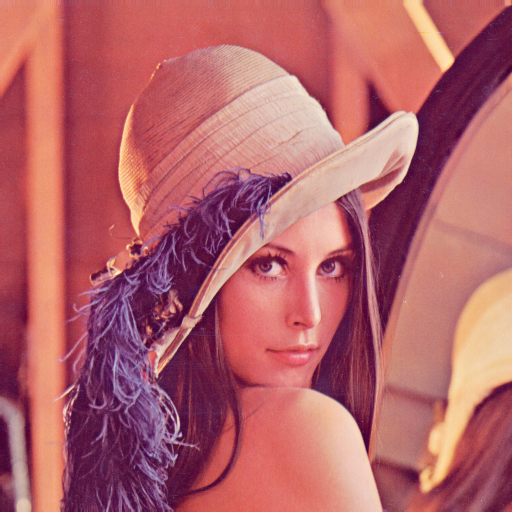
\includegraphics[width=2in]{lena512.png}\qquad
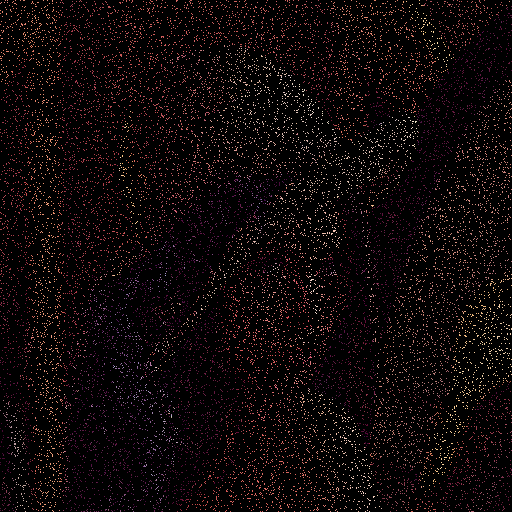
\includegraphics[width=2in]{lena512-random-mask-1.png}\qquad
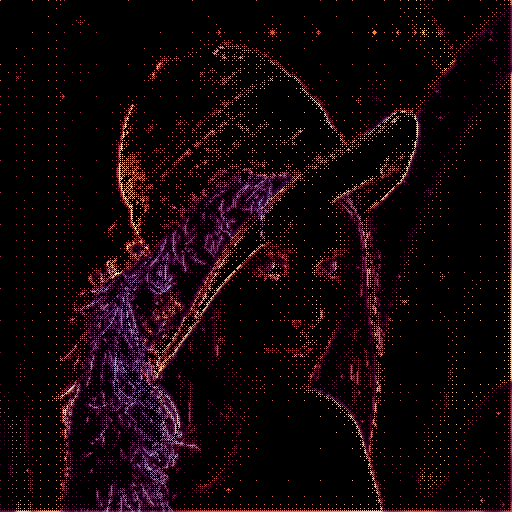
\includegraphics[width=2in]{lena512-bttc-mask-1.png}
\caption{Random vs. BTTC sample selection. For lena512.png, both images are sampled at $\approx 7.62\%$ of the total pixel count. The left image is generated with uniform random sampling. For BTTC on the right, we chose $\epsilon = 0.15$. Note that the BTTC implementation selects dense clusters of points along important edge features in the image, while areas with minor gradients have relatively sparse sampling.}
\label{bttcselectionfig}
\end{center}
\end{figure*}

\subsection{PDE Decompression}
Our decompression scheme involves first initializing the sampled pixels as seed points on an empty image with the same dimensions as the initial image. For the remaining pixels on the image, we can either leave them as white pixels or interpolate based on our seed pixels. With an additional interpolation step in our initialization, our inpainting should converge faster. Both methods should converge to similar images after the inpainting process, but the interpolation can introduce additional artifacts into the image, especially when used with the nonlinear EED method. One interpolation scheme we implemented for initializing the empty pixels is to simply clone the nearest seed pixel. We compute the Delaunay triangulation on the seed point indices and then clone each empty pixel from the closest vertex. The result is a shaded Voronoi diagram based on the seed pixels.

We implemented three versions of PDE-based diffusion methods described previously: linear isotropic (homogenous), nonlinear isotropic (Perona-Malik), and nonlinear anisotropic (EED). Our implementation of the first two methods were based on our own interpretation of the numerical solutions described in \cite{galic} and \cite{peronamalik}. Our nonlinear anisotropic edge-enhancing diffusion implementation is adapted from a coherence filter implementation outlined in \cite{kroon}; the EED diffusion matrix is generated from a downloaded library function.

\begin{figure*}[!htb]
\begin{center}
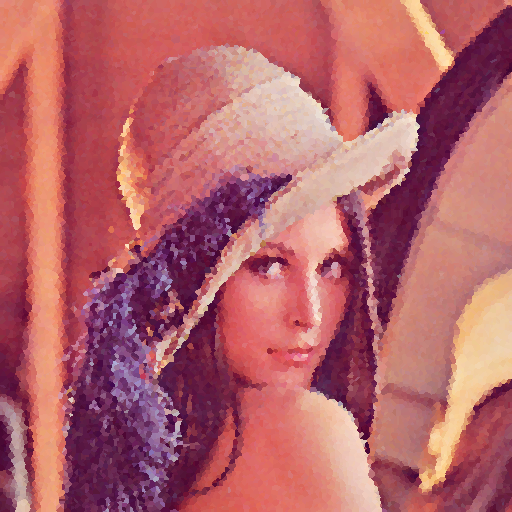
\includegraphics[width=2in]{lena512-random-voronoi-1}\qquad
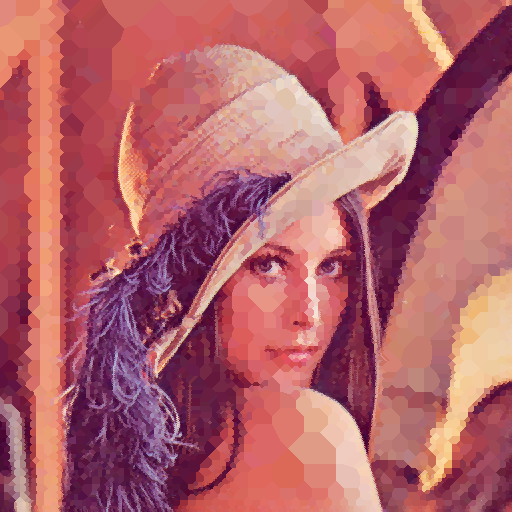
\includegraphics[width=2in]{lena512-BTTC-voronoi-1}\qquad
\includegraphics[width=2in]{castle512-BTTC-voronoi-1}
\caption{Initial Interpolation of Seed Pixels. A Delaunay triangulation is generated from the seed pixels, and the remain pixels are cloned after matching to a seed with a nearest neighbor search. The resulting image is effectively the Voronoi diagram of the seed points. From left to right, we have lena512 (random sampling), lena512 (BTTC sampling), castle512 (BTTC sampling) at $\epsilon = 0.25$ and $6.92\%$. Note that with BTTC, important features are more well defined.}
\label{voronoifig}
\end{center}
\end{figure*}

\subsection{Stopping Criteria}

Our goal is to estimate the steady state of the inpainting evolution $u(x,y,t)$ as $t \rightarrow \infty$ in finite time $T$.  The steady state occurs when $\partial_t u = 0$, and thus we want the stopping criteria to evaluate when change from one iteration to the next becomes small enough.  The threshold we use is the percentage of pixels deemed to be stable at a given time.  We define stability as a function
\begin{equation}
s(u^k, u^{k+1}) = \frac{1}{\Omega_{\text{dis}}} \sum_{(i,j) \in \Omega_{\text{dis}}} \phi(u_{i,j}^{k+1} - u_{i,j}^{k})
\end{equation}
where $\phi$ is the indicator function for whether the length of the input is below a value $\epsilon > 0$
\begin{equation}
 \phi(x) = \left\{
     \begin{array}{lr}
       1 & \text{if } ||x||_2 \leq \epsilon \\
       0 & \text{otherwise}
     \end{array}
   \right.
\end{equation}
Thus, $s(u^k, u^{k+1})$ returns the number of stable pixels divided by the total number of pixels at time $k+1$.  We choose a threshold proportion $p \in [0,1]$ such that we terminate iterations at time $k+1$ if $s(u^k, u^{k+1}) > p$.

\subsection{Measuring Error}
To measure the error, we will use mean-squared error (MSE).  For original image $v$ and approximation $u$, MSE is defined as
\begin{equation}
\text{MSE}(u,v) = \frac{1}{|\Omega_{\text{dis}}|} \sum_{j=1}^{N_1} \sum_{i=1}^{N_2} ||u(i,j) - v(i,j)||_2^2
\label{MSE}
\end{equation}
An alternative is the average-absolute difference (AAD), which is defined as,
\begin{equation}
\text{AAD}(u,v) = \frac{1}{|\Omega_{\text{dis}}|} \sum_{j=1}^{N_1} \sum_{i=1}^{N_2} ||u(i,j) - v(i,j)||_1
\label{AAD}
\end{equation}

\begin{figure*}[!htb]
\begin{center}
\includegraphics[width=2in]{./img/lena256.png}\qquad
\includegraphics[width=2in]{./img/lenaLI_0.png}\qquad
\includegraphics[width=2in]{./img/lenaLI_25.png}\\
\includegraphics[width=2in]{./img/lenaLI_50.png}\qquad
\includegraphics[width=2in]{./img/lenaLI_100.png}\qquad
\includegraphics[width=2in]{./img/lenaLI_200.png}\\
\includegraphics[width=2in]{./img/lenaLI_400.png}\qquad
\includegraphics[width=2in]{./img/lenaLI_800.png}\qquad
\includegraphics[width=2in]{./img/lenaLI_1600.png}\\
\includegraphics[width=2in]{./img/lenaLI_3200.png}\qquad
\includegraphics[width=2in]{./img/lenaLI_6400.png}\qquad
\includegraphics[width=2in]{./img/lenaLI_7050.png}\\
\caption{PDE image interpolation using linear isotropic diffusion. Image lena256.png (top left) is compressed using BTTC with $\epsilon = 0.2$ to $\approx 13.5\%$ of the total pixel count (top middle).  The image interpolation then evolves and is plotted at 10 iterations $k=\{25,50,100,200,400,800,1600,3200,6400,7050\}$.  These time steps are displayed starting from the top right.  The stability threshold for the algorithm is reached after 7050 iterations, so the bottom left picture gives the final result. The three diffusion methods have a similar convergence path, although the convergence speeds vary.}
\label{evolutionfig}
\end{center}
\end{figure*}
\pagebreak
\begin{figure*}[htb]
\begin{center}
\includegraphics[width=2in]{./img/lenaLI_diff_orig.png}\qquad
\includegraphics[width=2in]{./img/lenaLI_diff_0.png}\qquad
\includegraphics[width=2in]{./img/lenaLI_diff_25.png}\\
\includegraphics[width=2in]{./img/lenaLI_diff_50.png}\qquad
\includegraphics[width=2in]{./img/lenaLI_diff_100.png}\qquad
\includegraphics[width=2in]{./img/lenaLI_diff_200.png}\\
\includegraphics[width=2in]{./img/lenaLI_diff_400.png}\qquad
\includegraphics[width=2in]{./img/lenaLI_diff_800.png}\qquad
\includegraphics[width=2in]{./img/lenaLI_diff_1600.png}\\
\includegraphics[width=2in]{./img/lenaLI_diff_3200.png}\qquad
\includegraphics[width=2in]{./img/lenaLI_diff_6400.png}\qquad
\includegraphics[width=2in]{./img/lenaLI_diff_7050.png}\\
\caption{PDE image interpolation using linear isotropic diffusion.  Difference between the original image and the interpolated images displayed in Fig \ref{evolutionfig}. Black denotes areas of large differences while white denotes areas of small differences. Note that with the BTTC implementation, the interpolated image approximates the original image well at areas of high gradient.}
\label{evolutiondifffig}
\end{center}
\end{figure*}

\begin{figure*}[htb]
\begin{center}

\includegraphics[width=2in]{lena2.png}\qquad
\includegraphics[width=2in]{lena1.png}\\
\includegraphics[width=2in]{./img/lena-512-bttc-015-clean-max.png}\qquad
\includegraphics[width=2in]{./img/lena-512-bttc-015-clean-max-NL-1-100.png}\qquad
\includegraphics[width=2in]{./img/lena-512-bttc-015-clean-EED.png}
\caption{PDE interpolation convergence.  On the top, we have linear and nonlinear diffusion on the random pixel sampling. On the bottom, three diffusion methods are run on the image until convergence. Note that the edges are preserved much better. From left to right are the results for linear isotropic, nonlinear isotropic, and nonlinear anisotropic. MSE: 131.9 (Linear), 127.8 (Nonlinear), 127.7 (EED)}
\label{compfig}
\end{center}
\end{figure*}

\subsection{Comparison of Interpolation Methods}
The results for the three different diffusion techniques after convergence on BTTC points ($\epsilon = 0.15$) are displayed in Fig \ref{compfig}.  We can see that the results are pretty similar, but the image quality improves from left to right.  This is especially evident in the boundary of the image, where the linear isotropic contains some artifacts but these disappear in the nonlinear anisotropic.  The number of iterations until convergence also increases from left to right.  However, this comes at a tradeoff with time efficiency and simplicity.  Each iteration of the nonlinear anisotropic algorithm, for example, took over 10 times as long as an iteration for the linear isotropic.  All three methods had rapid convergence in solution, as show in Fig \ref{MSEFig}.
\begin{figure*}[hb]
\begin{center}
\includegraphics[width=5in]{./img/mse.eps}\qquad
\caption{MSE Convergence.}
\label{MSEFig}
\end{center}
\end{figure*}

\subsection{See MATLAB/README.txt}


%----------------------------------------------------------------------------------------
%	MATERIALS AND METHODS
%----------------------------------------------------------------------------------------

%% Optional Materials and Methods Section
%% The Materials and Methods section header will be added automatically.

%\begin{materials}
%Suspendisse viverra eleifend nulla at facilisis. Nullam eget tellus orci. Cras sit amet lorem velit. Maecenas rhoncus pellentesque orci eget vulputate. Phasellus massa nisi, mattis nec elementum accumsan, blandit non neque. In ac enim elit, sit amet luctus ante. Cras feugiat commodo lectus, vitae convallis dui sagittis id. In in tellus lacus, sed lobortis eros. Phasellus sit amet eleifend velit. Duis ornare dapibus porttitor. Maecenas eros velit, dignissim at egestas in, tincidunt lacinia erat. Proin elementum mi vel lectus suscipit fringilla. Mauris justo est, ullamcorper in rutrum interdum, accumsan eget mi. Maecenas ut massa aliquet purus eleifend vehicula in a nisi. Fusce molestie cursus lacinia.
%
%\begin{definition}
%A bounded function $\theta$ is a weak solution of QG if for any
%$\phi\,\epsilon\,
%C_0^{\infty}(\fdb\times\mathbb{R}\times[0,\vep])$ we have
%\begin{eqnarray}
%&&  \int_{\mathbb{R}^+\times\fd\times\mathbb{R}} \hspace{-25pt}
% \theta(x,y,t)\, \pr_t \phi
%\,(x,y,t) dy dx dt+\nonumber\\
%  & +&\int_{\mathbb{R}^+\times\fd\times\mathbb{R}}
%\hspace{-26pt} \theta\,(x,y,t) u(x,y,t)\cdot\nabla\phi\,(x,y,t)
%dydxdt = 0 \label{weaksol} \end{eqnarray}
%where $u$ is determined previously.
%\end{definition}
%
%Vestibulum ante ipsum primis in faucibus orci luctus et ultrices posuere cubilia Curae; Mauris eu sapien nunc, sit amet accumsan dui. Nulla ac diam ut nunc placerat semper eget et libero. Vestibulum ante ipsum primis in faucibus orci luctus et ultrices posuere cubilia Curae; Cras hendrerit ullamcorper sapien vitae luctus. Quisque vel diam massa. Vestibulum dui nibh, facilisis vel vestibulum eu, viverra in quam.
%
%\begin{theorem}
%If the active scalar $\theta$ satisfies
%the equation \eqref{weaksol}, then $\varphi$ satisfies the equation
%\begin{eqnarray}
%\mfrac{\pr \varphi}{\pr t}(x,t)&=&\hspace{-2pt}\dst
%\int_{\fd}\mfrac{\mfrac{\pr \varphi}{\pr x}(x,t)-\mfrac{\pr
%\varphi}{\pr
%u}(u,t)}{[(x-u)^{2}+(\varphi(x,t)-\varphi(u,t))^{2}]^{\f12}}\nonumber\\
%&&
%\chi(x-u,\varphi(x,t)-\varphi(u,t)) du \hspace{3pt} +
%\nonumber\\
%&+&\dst \int_{\fd} \Big{[}\mfrac{\pr \varphi} {\pr
%x}(x,t)-\mfrac{\pr \varphi}{\pr u} (u,t)\Big{]}
%\nonumber\\&&
%\eta(x-u,\varphi(x,t)-\varphi(u,t)) du + Error
%\end{eqnarray}
%with $|Error|\leq C\, \delta | log\delta| $ where $C$ depends only
%on $\|\theta\|_{L^{\infty}}$ and $\|
%\nabla\varphi\|_{L^{\infty}}$.
%\end{theorem}
%
%Class aptent taciti sociosqu ad litora torquent per conubia nostra, per inceptos himenaeos. Integer accumsan ornare tortor at varius. Phasellus ullamcorper blandit dolor sit amet tempus. Curabitur ligula urna, ultrices in iaculis eu, eleifend vel urna. Praesent ullamcorper imperdiet purus, ut interdum sem interdum dictum. Proin euismod volutpat eros ac mattis. Quisque sit amet massa ac tortor cursus malesuada at vitae nisi. Nam quis neque et nunc vehicula cursus sit amet at tellus.
%\end{materials}

%----------------------------------------------------------------------------------------
%	APPENDICES (OPTIONAL)
%----------------------------------------------------------------------------------------
%
%\appendix
%An appendix without a title.
%
%\appendix[Appendix title]
%An appendix with a title.
%
%----------------------------------------------------------------------------------------
%	ACKNOWLEDGEMENTS
%----------------------------------------------------------------------------------------
%
%\begin{acknowledgments}
%This work was partially supported by a grant from the Spanish Ministry of Science and Technology.
%\end{acknowledgments}

%----------------------------------------------------------------------------------------
%	BIBLIOGRAPHY
%----------------------------------------------------------------------------------------

%% PNAS does not support submission of supporting .tex files such as BibTeX.
%% Instead all references must be included in the article .tex document. 
%% If you currently use BibTeX, your bibliography is formed because the 
%% command \verb+\bibliography{}+ brings the <filename>.bbl file into your
%% .tex document. To conform to PNAS requirements, copy the reference listings
%% from your .bbl file and add them to the article .tex file, using the
%% bibliography environment described above.  

%%  Contact pnas@nas.edu if you need assistance with your
%%  bibliography.

% Sample bibliography item in PNAS format:
%% \bibitem{in-text reference} comma-separated author names up to 5,
%% for more than 5 authors use first author last name et al. (year published)
%% article title  {\it Journal Name} volume #: start page-end page.
%% ie,
% \bibitem{Neuhaus} Neuhaus J-M, Sitcher L, Meins F, Jr, Boller T (1991) 
% A short C-terminal sequence is necessary and sufficient for the
% targeting of chitinases to the plant vacuole. 
% {\it Proc Natl Acad Sci USA} 88:10362-10366.


%% Enter the largest bibliography number in the facing curly brackets
%% following \begin{thebibliography}

\begin{thebibliography}{10}
\bibitem{zimmer}
H.~Zimmer, {\em PDE-based image compression using corner information}, Master's Thesis, Dept. of Informatics and Mathematics, Saarland University, (2007).

\bibitem{jpeg}
Wikipedia, {\em JPEG}, Accessed December 15, 2003.

\bibitem{distasi}
R.~Distasi, M.~Nappi, and S.~Virtulano, {\em Image Compression by {BTTC}-Tree Triangular Coding}, IEEE Transactions on Communication, 45, 9 (1997).

\bibitem{galic}
I.~Galic, J.~Weikert, et al, {\em Towards PDE-based Image Compression}, In N. Paragios, O. Faugeras, T. Chan, C. Schn�rr (Eds.): Variational, Geometric, and Level Set Methods in Computer Vision. Lecture Notes in Computer Science, Vol. 3752, Springer, Berlin, 37-48, 2005.

\bibitem{weickertEED}
J.~Weickert and H.~Scharr, {\em A Scheme for Coherence-Enhancing Diffusion
Filtering with Optimized Rotation Invariance}, Journal of Visual Communication and Image Representation 13, 103�118 (2002)

\bibitem{galic2}
I. Galic, J. Weickert, M. Welk, A. Bruhn, A. Belyaev, H.-P. Seidel,{
Image compression with anisotropic diffusion},
Journal of Mathematical Imaging and Vision, Vol. 31, 255�269, 2008. Invited Paper.

\bibitem{weickert2}
Weickert, J. {\em Anisotropic Diffusion in Image Processing}. B.G. Teubner, Stuggart (1998).

\bibitem{kroon}
D.~Kroon, {\em Image Edge Enhancing Coherence Filter Toolbox}, Matlab Toolbox, (2010),
http://www.mathworks.com/matlabcentral/fileexchange/25449-image-edge-enhancing-coherence-filter-toolbox.

\bibitem{peronamalik}
P. Perona, J. Malik, {\em Scale-Space and Edge Detection Using Anisotropic Diffusion},
IEEE Transactions on Pattern Analysis and Machine Intelligence, 12(7):629-639, July 1990.
  
\end{thebibliography}

%----------------------------------------------------------------------------------------

\end{article}

%----------------------------------------------------------------------------------------
%	FIGURES AND TABLES
%----------------------------------------------------------------------------------------

%% Adding Figure and Table References
%% Be sure to add figures and tables after \end{article}
%% and before \end{document}

%% For figures, put the caption below the illustration.
%%
%% \begin{figure}
%% \caption{Almost Sharp Front}\label{afoto}
%% \end{figure}

%\begin{figure}[h]
%\centerline{\includegraphics[width=0.4\linewidth]{placeholder.jpg}}
%\caption{Figure caption}\label{placeholder}
%\end{figure}

%% For Tables, put caption above table
%%
%% Table caption should start with a capital letter, continue with lower case
%% and not have a period at the end
%% Using @{\vrule height ?? depth ?? width0pt} in the tabular preamble will
%% keep that much space between every line in the table.

%% \begin{table}
%% \caption{Repeat length of longer allele by age of onset class}
%% \begin{tabular}{@{\vrule height 10.5pt depth4pt  width0pt}lrcccc}
%% table text
%% \end{tabular}
%% \end{table}

%% For two column figures and tables, use the following:

%% \begin{figure*}
%% \caption{Almost Sharp Front}\label{afoto}
%% \end{figure*}

%% \begin{table*}
%% \caption{Repeat length of longer allele by age of onset class}
%% \begin{tabular}{ccc}
%% table text
%% \end{tabular}
%% \end{table*}

%----------------------------------------------------------------------------------------

\end{document}